\documentclass{article}%
\usepackage[T1]{fontenc}%
\usepackage[utf8]{inputenc}%
\usepackage{lmodern}%
\usepackage{textcomp}%
\usepackage{lastpage}%
\usepackage[head=40pt,margin=0.5in,bottom=0.6in]{geometry}%
\usepackage{graphicx}%
%
\title{\textbf{Gobierno incrementa persecución a periodistas}}%
\author{SOFÌA NEDERR}%
\date{28/09/2018}%
%
\begin{document}%
\normalsize%
\maketitle%
\textbf{URL: }%
http://www.el{-}nacional.com/noticias/politica/gobierno{-}incrementa{-}persecucion{-}periodistas\_253532\newline%
%
\textbf{Periodico: }%
EN, %
ID: %
253532, %
Seccion: %
Política\newline%
%
\textbf{Palabras Claves: }%
Libertad de expresión, Sociedad\newline%
%
\textbf{Derecho: }%
1.7, %
Otros Derechos: %
, %
Sub Derechos: %
\newline%
%
\textbf{EP: }%
SI\newline%
\newline%
%
\textbf{\textit{Piden a la Defensoría que inste a la Fiscalía a procurar las acciones para reponer los derechos vulnerados, establecer responsabilidades y aplicar sanciones. También solicitan reunirse con los jefes de la GN, PNB y el Sebin para que cumplan sus obligaciones de respetar los derechos y garantías constitucionales de los reporteros~}}%
\newline%
\newline%
%
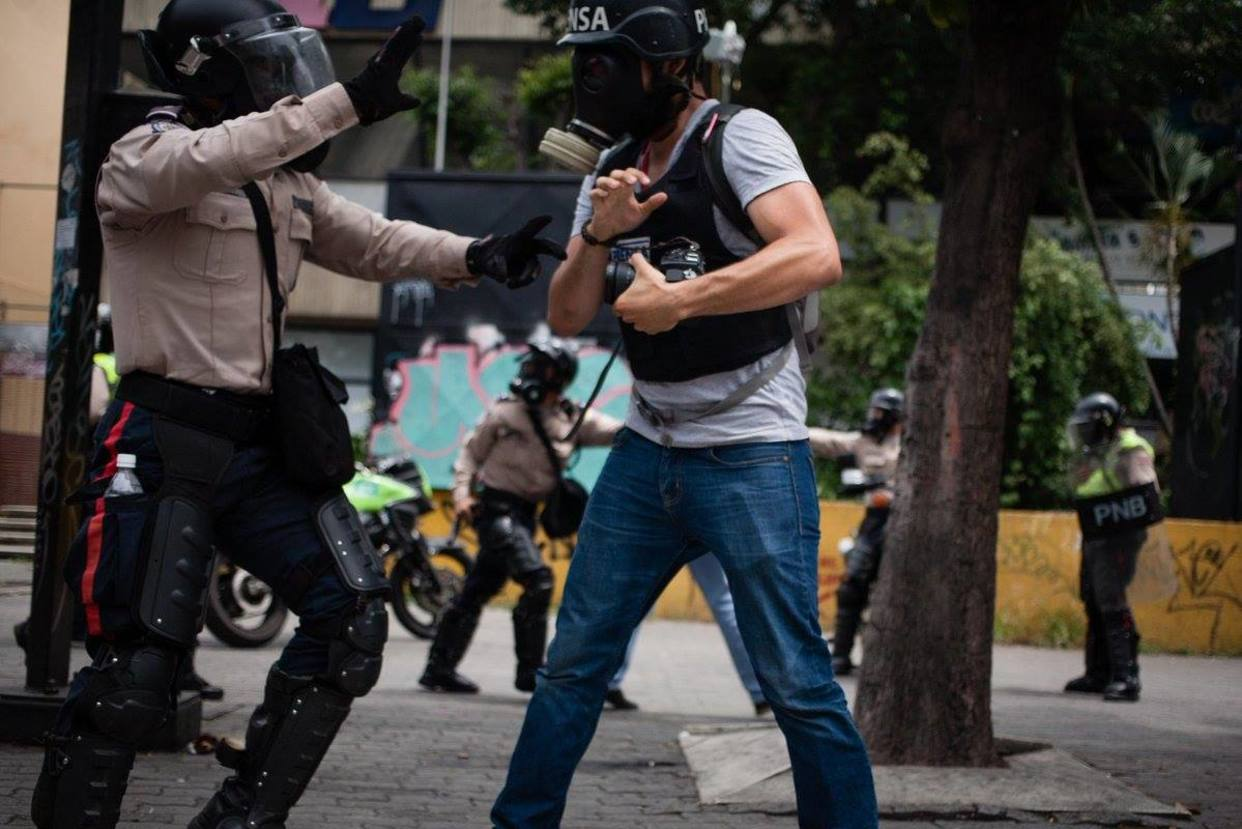
\includegraphics[width=300px]{26.jpg}%
\newline%
%
La persecución a los periodistas y a los medios independientes en Venezuela ha arreciado en los últimos días dado que el plan del gobierno es impedir que se conozca la magnitud de la crisis del país, advierten el Colegio Nacional de Periodistas, Espacio Público y el Instituto de Investigaciones de la Comunicación de la UCV.%
\newline%
%
“El gobierno no quiere que se sepa lo que ocurre. Frena la difusión de noticias, con lo que vulnera la libertad de expresión, y busca que se conozca solo la versión de los voceros ministeriales que no tienen credibilidad, quienes aseguran que en el país no pasa nada”, dijo el~presidente del CNP, Tinedo Guía.%
\newline%
%
Repudió el patrón de ataques que incluye la anulación de pasaportes como ocurrió con Nelson Bocaranda; los arrestos arbitrarios durante la cobertura noticiosa, que son los casos del reportero Rey Mozo, que cubría la llegada del buque chino con asistencia humanitaria; la detención y las limitaciones a la información impuestas a Isnardo Bravo; la agresión con un cuchillo a un equipo de VPI y los obstáculos a la reseña de hechos como las inundaciones en el Orinoco, entre otros casos.%
\newline%
%
“Las limitaciones impuestas son de forma personal contra periodistas y también contra los medios independientes como ocurre con el papel periódico”, añadió.%
\newline%
%
Sostuvo que el gobierno ahora emplea el Saime para atacar o presionar a los periodistas. En esto coincide Luisa Torrealba, coordinadora del Ininco. El mecanismo empleado para perseguir o amedrentar ya no solo se lleva a cabo con la utilización de los organismos de seguridad o de acciones judiciales: las agresiones que se han hecho a través del Saime también han afectado a los familiares y todo el entorno de los periodistas, que son el blanco de la persecución.%
\newline%
%
“Es muy grave lo que ocurre con los comunicadores que son acosados. En estos casos hay intimidación, violencia y censura. A su vez, estos hechos generan autocensura y, en algunos casos, los periodistas una vez que han resuelto su situación, abandonan el país”, señaló Torrealba.%
\newline%
%
Agregó que cada vez más se observa la presión del gobierno para limitar que se difunda la información que no le conviene y se imponga un discurso, un mensaje único.%
\newline%
%
Recordó que el problema del papel no solo afecta a los diarios de circulación nacional, igualmente perjudica a los medios de las regiones: “Con el agravante de que hay estados donde no queda ningún periódico, esto pese a que se anuncia la salida como temporal”.%
\newline%
%
La investigadora afirmó que se aprecia un bloqueo selectivo con la disminución de la publicidad oficial y se limita a las emisoras de radio, la mayoría de las cuales no tienen noticieros.%
\newline%
%
“En el país se viola el derecho a la libertad de expresión, el derecho a la libertad de información; el derecho a la información pública y el derecho a la libertad de conciencia. Todo esto ocurre mientras se incrementan mecanismos de control social como el carnet de la patria”, denunció.%
\newline%
%
Carlos Correa, director de Espacio Público, dijo: “Las recientes agresiones son una vuelta de tuerca de la política sostenida del Estado contra la libertad de expresión\&mldr; Esto se evidencia en los casos de Nelson Bocaranda, de Isnardo Bravo y de otros periodistas, pero también en el de los bomberos de Mérida y del ciudadano que está detenido por informar, en Twitter, sobre la ruta del avión presidencial”.%
\newline%
%
Correa agregó que los bloqueos contra portales web siguen y se acentúa el hostigamiento mediante dictámenes judiciales que buscan la reparación económica, tras las demandas interpuestas contra~El Nacional~y~La Patilla,~por presunta difamación.%
\newline%
%
El Sindicato Nacional de Trabajadores de la Prensa alertó que “el vicepresidente del PSUV, Diosdado Cabello, amenaza con quedarse con~El Nacional~y~La Patilla, a propósito de la decisión de un juez que habría fallado en su favor en una demanda contra el portal digital de noticias y la anterior contra el diario”.%
\newline%
%
Contra la impunidad. Carlos Correa afirmó que la carta entregada hoy ante la Defensoría del Pueblo es la segunda que se envía a su titular, Alfredo Ruiz, para que “resguarde los derechos de los periodistas y medios de comunicación debido a que persiste una política claramente restrictiva”.%
\newline%
%
Piden al defensor que inste a la Fiscalía General a que procure las acciones y los recursos para reponer los derechos vulnerados, establezca las responsabilidades y aplique sanciones. También solicitan una reunión conjunta con los comandantes de la Guardia Nacional, la Policía Nacional Bolivariana y el Sebin “para imponerlos de su obligación de respetar los derechos y garantías constitucionales de los periodistas, nacionales y extranjeros, con el fin de evitar que continúen las obstrucciones a su labor informativa”.%
\newline%
%
La carta fue remitida por la Alianza para la Libertad de Expresión, integrada por el Centro de Derechos Humanos de la Universidad Católica Andrés Bello; el Colegio Nacional de Periodistas; el Comité por una Radiotelevisión de Servicio Público;~Espacio Público; Expresión Libre; la Federación Venezolana de Estudiantes de Comunicación Social; el Instituto de Investigaciones de la Comunicación de la UCV; IPYS Venezuela, y~Ser Investigación y Comunicación.%
\newline%
%
\end{document}